\chapter{System Architectural Design}

\section{System Components}



This chapter seeks to identify the system components. It provides a block definition diagram (bdd) of the system, where the system components are determined along with the static relationship between them. The block definition diagram is shown in figure \ref{fig:block_diagram}:

\begin{figure}[H]
\centering
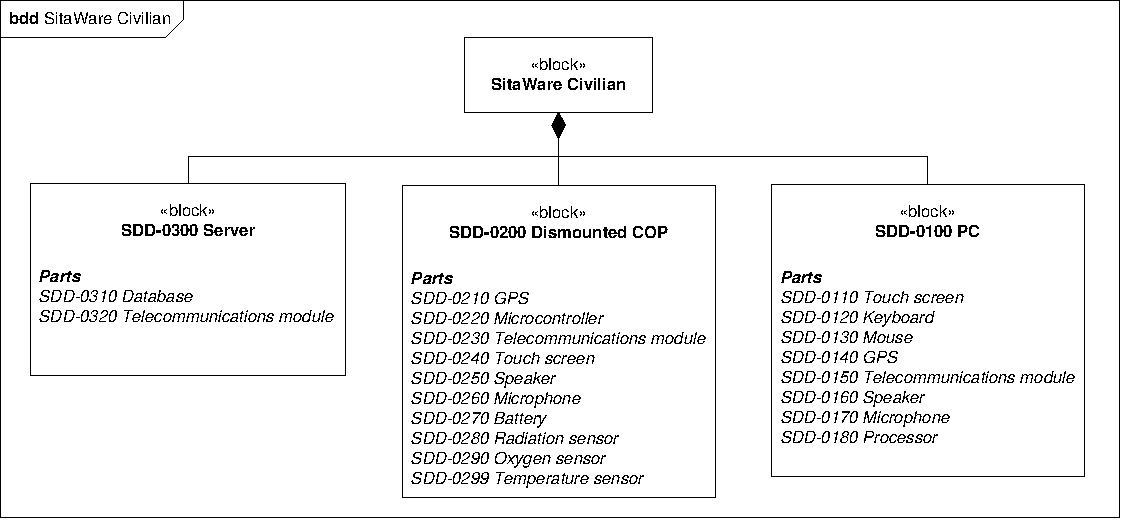
\includegraphics[width=0.95\textwidth]
{billeder/bdd_overordnet.pdf}
\caption{Block diagram of the system.}
\label{fig:block_diagram}
\end{figure}

The diagram consists of system-blocks along with parts associated to each block. The system-blocks are depicted as two-compartment blocks with the name of the block in the first compartment, and sub parts in the second compartment. In the next section, a short description of each system-block is given.

\subsection{Component description}
\begin{enumerate}
\item[•] \textbf{PC:} This block constitutes the machine in the head quarter (HQ) on which the COP-software will be executed. It also has a GPS module, so that the location of the HQ is always known. The PC has a telecommunication module, in order to be able to communicate with the rest of the system.
\item[•] \textbf{Server:} The server will facilitate communication between the other blocks. In addition, it will store user information along with logs locally in an internal database.
\item[•] \textbf{Dismounted COP:} This block constitutes the machine on which the condensed COP-software will be executed. The dismounted COP will be used by the dismounted users in the field. It has a GPS module, so that the location of the dismounted users is always known. Furthermore it has a telecommunication module so that it will be able to communicate with the rest of the system. 
\end{enumerate}
\section{Concept of Execution}

\section{Interface Design}

\subsection{PC}
When looking into the PC the different modules are displayed on the ibd. The connections between the modules describes the data flow. In the PC a processor is connecting all the units together, while the telecommunication module is connecting the PC to the other devices. The i/o from the microphone, speakers, touch screen, mouse and keyboard reaches to the physical world to connect with the user.


\section{Concept of execution}

\begin{figure}[H]
\centering
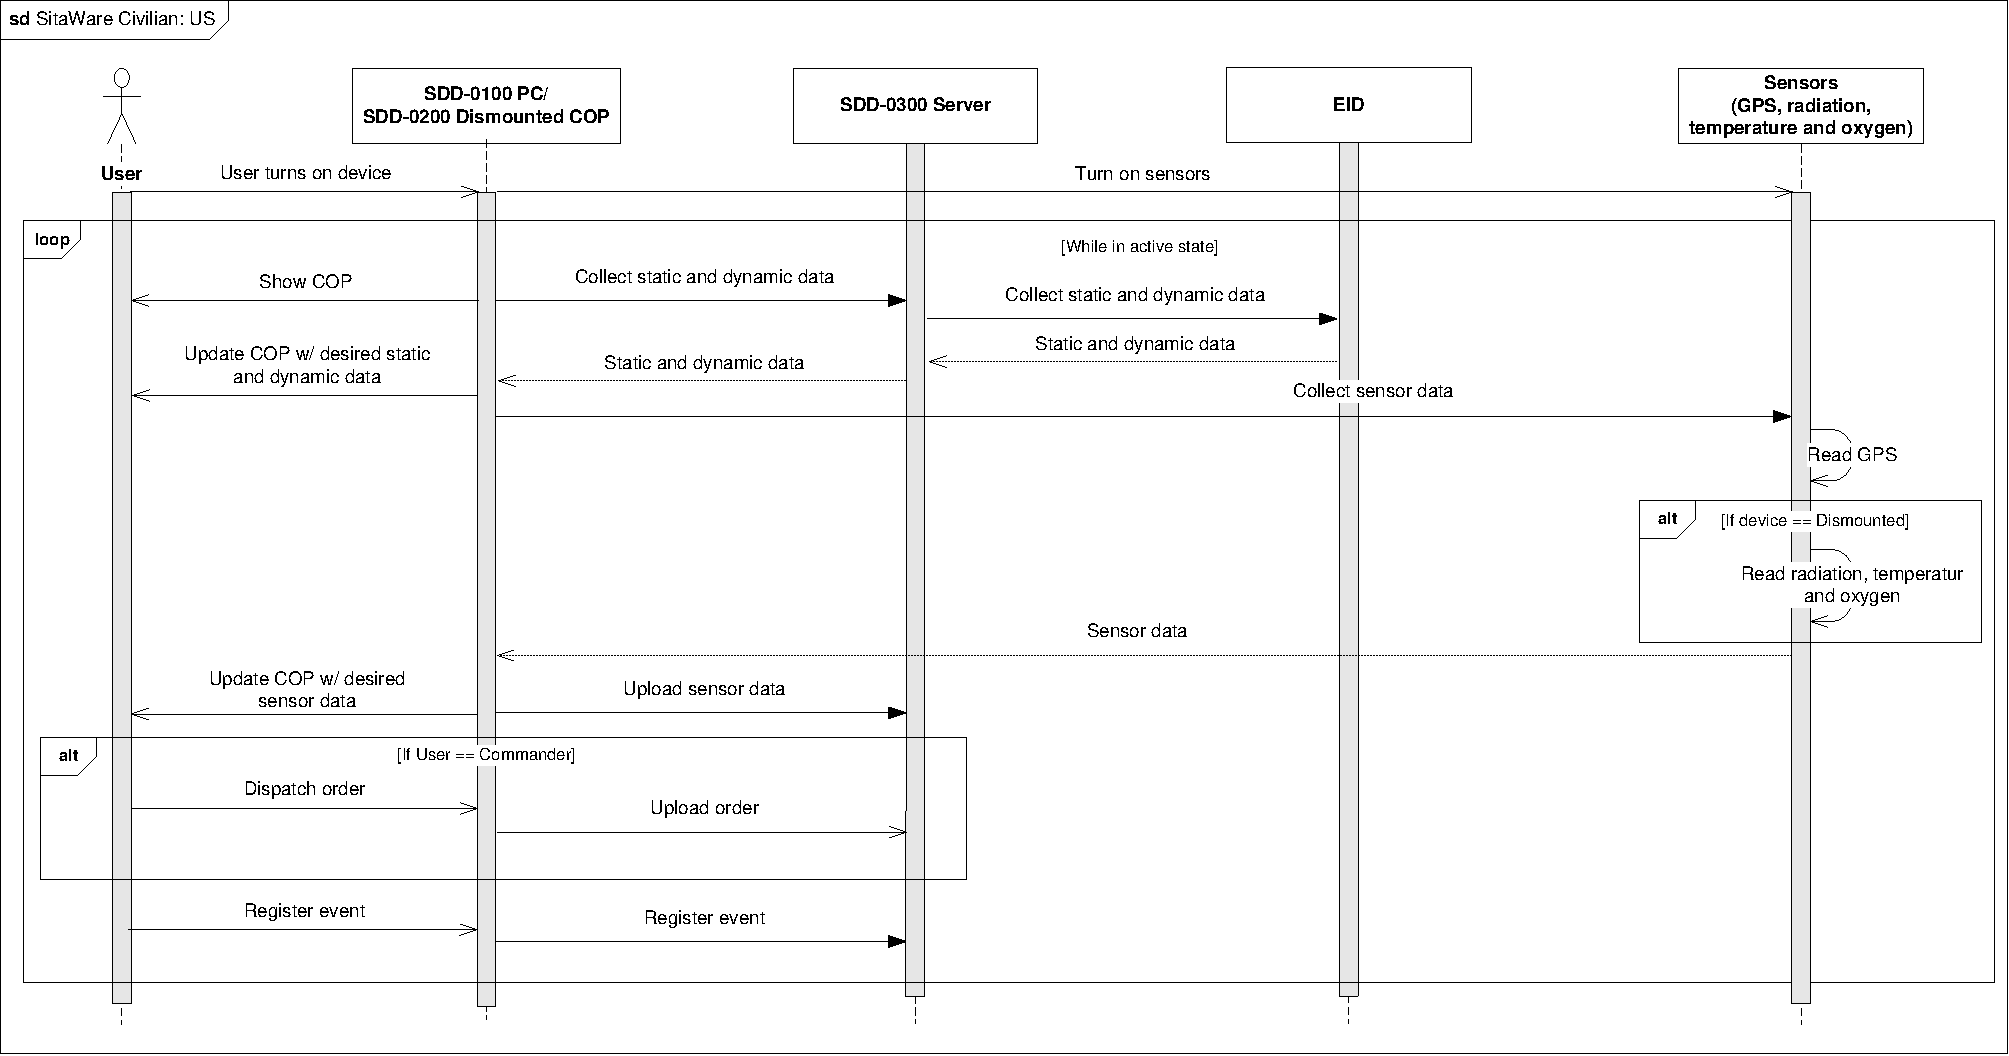
\includegraphics[width=0.95\textwidth]
{billeder/sekvens1.pdf}
\caption{Overall sequence diagram for SitaWare Civilian.}
\label{fig:sekvens1}
\end{figure}